\documentclass[11pt]{article}

\newcommand{\numpy}{{\tt numpy}}    % tt font for numpy

% for symbols
\usepackage{bbold}
\usepackage{amsmath,amssymb}
\DeclareMathOperator*{\argmin}{arg\,min}
\DeclareMathOperator*{\argmax}{arg\,max}
\setlength\parindent{15pt}

% for images
\usepackage{graphicx}
% \graphicspath{ {./images/} }


\DeclareRobustCommand{\bbone}{\text{\usefont{U}{bbold}{m}{n}1}}
\DeclareMathOperator{\EX}{\mathbb{E}}% expected value

\topmargin -.5in
\textheight 9in
\oddsidemargin -.25in
\evensidemargin -.25in
\textwidth 7in

\begin{document}

% ========== Edit your name here
\author{Monika, Jordi and Sebastian}
\title{Stochastic Modelling and Optimisation - Final Project}
\maketitle

\medskip

% ========== Begin answering questions here
\section{Introduction}
Nobody likes traffic. Traffic decreases the productivity of urban spaces, and translates into lower prosperity. Controlling the amount of traffic is therefore a priority goal for urban planners. Yet, most cities face natural or financial constraints in the expansion of transport networks. Consequently,  urban planners are faced with the challenge of optimising traffic flows within the constraints of existing infrastructure, to ensure the most efficient use of it possible.

In this project we study how dynamic programming can be applied to optimise traffic flows. Specifically, we employ the traffic response urban control (TUC) strategy initially proposed by Diakaki, Papageorgiou, & McLean (1999). 


\section{DP formulation}
\subsection{Variable definitions}
\begin{tabular}{ l l c }
Links (approaches): & $z \in Z$  &\\
Junctions: & $j \in J$ &\\
Set of inflowing links: & $I_j$ &\\
Set of outflowing links: & $O_j$ &\\
Cycle time (We assume $C_j = C$ for all junctions) : & $C_j$ & \\
Total lost time: &$L_j$ &\\
Set of stages: & $F_j$ &\\
Set of stages where link z has r.o.w.: & $v_z$ &\\
Saturation flow for link z: & $S_z$ &\\
Turning rates for inflowing link z and outflowing link w: & $t_{z,w}$ &\\
Green time of stage i at junction j: & $g_{j,i}$ &\\
Control interval: & $T$ &\\
Period intervals: & $[k T,(k+1) T]$ &\\
Demand flow: & $d_z$ &\\
Exit flow: & $ s_z $ &\\
\end{tabular}

\subsection{Constraints and indentities}
\begin{tabular}{ l l }
Green light constraints: & $g_{j,i} \in \left[g_{j, i, \min }, g_{j, i, \max }\right]$ \\
Cycle time constraint: & $\sum_{i \in F_{j}} g_{j, i}+L_{j}=C$ \\
Exit flow constraint: & $s_{z}(k)=t_{z, 0} q_{z}(k)$ \\
Inflow to link z: & $q_{z}(k)= \sum_{w \in I_{M}} t_{w, z} u_{w}(k)$ \\
Outflow from link z: & $u_z = \left\{ \begin{array} { l l } { S_z } & { \text { if  has r.o.w}  } \\ { 0 } & { \text { otherwise} } \end{array} \right.$ \\
(Assuming space available in downstream link and $x_z>S_z$\\
Average value for outflow from z: & $u_{z}(k)=S_{z} G_{z}(k) / C$\\
Effective green time: & $G_{z}(k)=\sum_{i \in v} g_{j, i}(k)$ \\
Steady state demand: & $\left(1-t_{z, 0}\right) q_{z}^{N}+d_{z}^{N}-u_{z}^{N}=0$ \\
(Assuming nominal green times that lead to steady-state \\
link queues under non-saturating constant nominal demand) \\
\end{tabular}


\subsection{DP equations}
\subsubsection*{Dynamics:}
\begin{equation}
x_{z}(k+1)=x_{z}(k)+T\left[q_{z}(k)-s_{z}(k)+d_{z}(k)-u_{z}(k)\right]
\end{equation}
Substituting gives:
\begin{equation}
x_{z}(k+1) =x_{z}(k)+T\left[\left(1-t_{z, 0}\right) \sum_{w \in I_{M}} \frac{t_{w, z} S_{w}\left(\sum_{i \in v_{w}} \Delta g_{M, i}(k)\right)}{C} +\Delta d_{z}(k)-\frac{S_{z}\left(\sum_{i \in v_{z}} \Delta g_{N, i}(k)\right)}{C} \right]
\end{equation}
In vector notation: 
\begin{equation}
\mathbf{x}(k+1)=\mathbf{A} \mathbf{x}(k)+\mathbf{B} \Delta \mathbf{g}(k)+\mathbf{T} \Delta \mathbf{d}(k)
\end{equation}
where $ \mathbf{x} $ is the state vector of the numbers of vehicles $ \mathbf{x}_z$ within links $z \in Z$ and $\Delta g_{j, i}=g_{j, i}-g_{j, i}^{\mathrm{N}}$ is the vector of deviations from the steady-state green times and $\Delta d_{z}=d_{z}-d_{z}^{\mathrm{N}}$ is the deviation from the steady-state demand flows. $\mathbf{A}= \mathbf{I}$, $\mathbf{B}$ and  $\mathbf{T}$ are the state, input, and disturbance matrices, respectively. The input matrix B reflects the specific network topology, fixed staging, cycle, saturation flows, and turning rates. For this problem we assume demand is in its steady-state: $\Delta \mathrm{d}(k)=0$.
\subsubsection*{Cost:}
\begin{equation}
\mathcal{J}=\frac{1}{2} \sum_{k=0}^{\infty}\left(\|\mathbf{x}(k)\|_{\mathbf{Q}}^{2}+\|\Delta \mathbf{g}(k)\|_{\mathbf{R}}^{2}\right)
\end{equation}
Here $\mathbf{Q}$ and $\mathbf{R}$ are non-negative definite, diagonal weighting matrices. The infinite sum in the equation (4) suggest an infinite time horizon, which is taken in order to obtain a time-invariant feedback law according to the LQ optimisation theory. Intuitively,  the first term in (4), $\|\mathbf{x}(k)\|_{\mathbf{Q}}^{2}$ is responsible for minimisation and balancing of the relative occupancies of the network links. $\mathbf{Q}$ is defined as a diagonal matrix with the diagonal elements equal to the inverses of the storage capacities of the corresponding links. Lastly, matrix $\mathbf{R}$ influences the magnitude of the control reactions. Therefore,  $\mathbf{R}=r\mathbf{I}$, where the choice of r is picked to ensure the best results for a given application network (i.e. simple trial-error procedure).

\subsubsection*{Solution:}
The aim of this problem is to minimise the cost presented in equation (4) subject to constraints in (3). Having recognised the problem as a discrete-time linear quadratic control problem with and infinite-horizon subject to state equation (3), one can make use of an algebraic Riccati equation to find the solution.\\

We define a symmetric positive definite \textbf{cost-to-go matrix X} evolving backwards in time from $X _ { T } = Q$ according to:
\begin{equation} 
X _ { k - 1 } = Q + A ^ { T } X _ { k } A - A ^ { T } X _ { k } B \left( B ^ { T } X _ { k } B + R \right) ^ { - 1 } B ^ { T } X _ { k } A
\end{equation}
which is known as the discrete-time dynamic Riccati equation of this problem. The steady-state characterization of X, relevant for the infinite-horizon problem in which T goes to infinity, can be found by iterating the dynamic equation repeatedly until it converges; then X is characterized by removing the time subscripts from the dynamic equation. Resulting in:
\begin{equation}
X = Q+ A ^ { T } X A - \left( A ^ { T } X B \right) \left( R + B ^ { T } X B \right) ^ { - 1 } \left( B ^ { T } X A \right)
\end{equation}


Solution to this problem is therefore given by a matrix (called the control) $\mathbf{L}$:
\begin{equation}
\mathbf{L} = \left(B ^ { T } X B +R \right) ^ { - 1 } B ^ { T } X A % other notations use K and I m not sure if thats the same as our L :( 
\end{equation}

Putting it into DP framework that uses backwords induction, the optimal control solution at each time k is equivalent to:
\begin{equation} 
\Delta g _ { k } ^ { * } = - \left( B ^ { T } X _ { k } B + R \right) ^ { - 1 } \left( B ^ { T } X _ { k } A \right) x _ { k - 1 }
\end{equation}

Dropping the k's because of the infinite horizon assumption, the equation transforms to:

\begin{equation} 
\Delta g  ^ { * } = - \left( B ^ { T } X  B + R \right) ^ { - 1 } \left( B ^ { T } X  A \right) x _ { k - 1 }
\end{equation}

And can equivalently by written as:
\begin{equation} 
\mathbf { g } ( k ) = \mathbf { g } ^ { \mathrm { N } } - \mathbf { L } \mathbf { x } ( k )
\end{equation}
where $\Delta \mathbf {g } = \mathbf { g } ( k ) - \mathbf {g } ^ { \mathrm { N } }$.\\


The optimasation of this network is not done yet. This is because the LQ problem presented above does not consider control constraints. Those, however, can be imposed after the solution to (9) is computed. Hence, this calls for another optimasation problem that is solved in real-time forfor each junction $j$ so as to specify feasible green times $G _ { j , i }$ that are closest in distance to the non-feasible regulator-based green times $g _ { j , i }$ resulting from (9).


\begin{equation} \operatorname { min } { G _ { j , i } } \sum _ { i \in F _ { j } } \left( g _ { j , i } - G _ { j , i } \right) ^ { 2 }\end{equation} 
subject to
\begin{equation} 
\sum _ { i \in F _ { j } } G _ { j , i } + \left| L _ { j } = C \right.
\end{equation} 
\begin{equation} 
G _ { j , i } \in \left[ g _ { j , i , \min } , g _ { j , i , \max } \right] \forall i \in F _ { j }
\end{equation} 


\begin{figure}
    \caption{Network Graph}
      \centering
	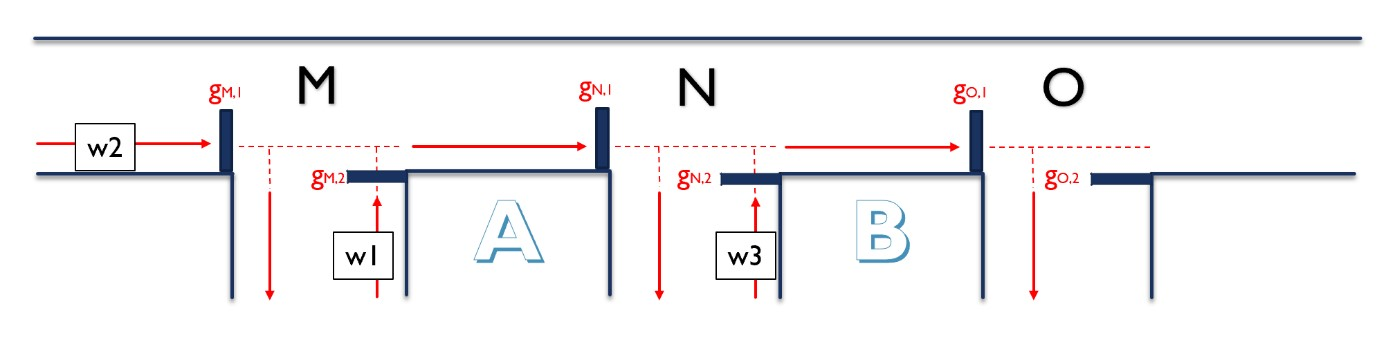
\includegraphics[width=15cm]{network-graph}
\end{figure}


% ========== Continue adding items as needed

\end{document}
\grid
\grid